\chapter{微分学}
\section{微分学的基本思想}

\noindent\textbf{1. 新的历史条件与新的要求}\quad
我们在第一章中就已讲到，关于运动和变化的考察从古希腊就已开始，而且由芝诺、毕达哥拉斯到欧多克萨斯、欧几里得，不论是在哲学的思辨上或者在数学基础上都达到了很高的水平。但是，不但有这些纯思辨的考察，还有许多有待解决的实际问题，推动着科学的进步。从当时的生产力发展的一般水平以及与之相应的科学技术发展水平来看，静力学、流体的静力学、光学，特别是物体的机械运动，包括地上的和天上的物体的运动都是当时科学发展中的关键问题，其中一个重大问题是天体运行规律问题。

由古希腊的托勒密地心说以至后来哥白尼的日心说，以至布鲁诺被施以火刑、伽利略受到教廷的迫害，我们时常看到的是它的意识形态方面。但是这个问题的意义远不止此，现在每一个中学生都懂得了什么是相对运动，那么，日心说与地心说之差别无非是采用了不同的坐标系，何必大动干戈呢？但是能把问题“看穿”到这个地步，前提是要能用数学很好地刻画运动，要能追踪星体在天空运动的轨迹，写出其运动方程式，而不是只满足于亚里士多德式的思辨，说什么物体下坠是因为向下落是物体“自然的本性”之类。这就不但不是依赖哲学，而恰好是能摆脱某种哲学，回到科学的道路上，回到观测、推算等等科学方法的道路上。不仅是天体运动的规律，还有关于运动学的基本概念如速度、加速度如何理解，什么是力，什么是离心力等等都是16--17世纪前后科学界关心的焦点。牛顿力学三大定律正是在这样的科学氛围中出现的。它一方面吸收了许多人，特别是伽利略、笛卡儿的成就，另一方面自然也是牛顿本人的努力和天才的结晶。所以牛顿说自己是站在巨人肩上是很有道理、很有见解的。我们特别要提出，牛顿深受欧几里得《几何原本》的影响，在他的巨著《自然哲学之数学原理》（1686，以下简称《原理》，中译本，武汉出版社，1992）一书中，他就把三大定律列为“运动的公理或定律”并由此推出《原理》中所有的命题。这一点确实是牛顿的伟大贡献。

可是，这一切努力绝不是只具有理论的兴趣，而要实际得多。例如，由于资本主义向全世界的扩展，人们需要作长距离的航海，而确定船只在海洋中的位置自然是重要的。确定纬度比较容易，只要测定某一个恒星离天顶的角度即可，但确定经度却要困难得多。大约从16世纪起，人们就开始利用时差来确定经度。但为此，一是要有关于天体运动的准确知识，1675英王查理二世建立格林尼治天文台，就是为了这个目的。研究天体运动的人不仅有伽利略和牛顿，还有许多人，其中例如有哈雷（Edmund Halley，1656--1742，哈雷彗星的发现者），他所作的星图是最精确的。二是要有一个好的钟。单摆是当时人们测定时间的基本工具。关于单摆的研究工作的基础是由惠更斯和胡克（Robert Hooke，1635--1703，曾任英国皇家学会秘书，与牛顿为了万有引力定律的“知识产权”闹过不小的矛盾）奠定的。但是为了计算经度，摆的误差每天不得超过2--3秒，这在当时是很难达到的。由此还产生过一次灾难：1707年，一支由5艘军舰组成的英国舰队，在海军元帅叔莱尔（Admiral Sir Cloudesley Shovell）\jiaokan{原文英文名作“Admiral Sir Clawdisley Shorell”。1707年锡利海难中英国舰队指挥官为 Sir Cloudesley Shovell（1650--1707），今据通行写法改正英文名。}率领下在直布罗陀大败法国舰队。可是在凯旋回国时遇大雾，因无法确定舰队准确位置而触礁，五艘军舰沉没了四艘，死亡水兵二千余人。在举国大哗之下，英国国会于1714年通过“经度法案”，悬赏20 000英镑（约合今天\$1 000 000），征求确定经度之法，最后由一位哈里逊（John Harrison，1693--1776）在1761年造出了可以实用的海钟（当时称为 chronometer）而获奖。哈里逊没有读过大学，是一位极为能干的工匠。（以上见于 N. F. Lane, Problem Solving in Complex Society, AMS, Notices, Vol.44, May (1997), 580--584）。总之，微积分发展的环境已与希腊时代和中世纪有了天壤之别。

关于天体的运动——当时还主要是太阳系中行星运动的规律。由于问题的重要性，人们已经进行了多年的观测，积累了大量观测数据。到17世纪初，开普勒以多年观测数据为基础，提出了著名的开普勒三定律。

\noindent I．开普勒第一定律：行星运行的轨道是椭圆，太阳位于椭圆的一个焦点上。

\noindent II．开普勒第二定律：联结太阳和某行星的线段称为行星的动径。若采用极坐标，令太阳在原点处，动径就是一个向量 $\boldsymbol r$。在相同时间内，$\boldsymbol r$ 扫过的扇形面积相同。简单的说法就说各行星的面积速度是一个常数（当然，不同的行星之面积速度是不同的常数）。

\noindent III．开普勒第三定律：各行星的周期各不相同，但是周期 $T$ 与轨道椭圆的长半轴 $a$ 之 $3/2$ 次方成正比，即
\[
\frac{T}{a^{3/2}}=\mathrm{const},
\]
注意，这个常数适用于各个行星。

开普勒三定律是唯象定律，它没有解释为什么恰好有这三个定律成立。牛顿的功绩在于指出了，它们其实是一个更深刻的定律：万有引力定律的推论。万有引力定律指出，若有二质点，质量各为 $m_1$ 与 $m_2$，设一个质点在极坐标原点处，另一质点的动径为 $\boldsymbol r$，则第一质点对另一质点必有引力，其方向与 $-\boldsymbol r$ 相同，而大小则与 $r^2$ 成反比，或者写成
\[
\boldsymbol F=-G\frac{m_1m_2}{r^2}\frac{\boldsymbol r}{r},\qquad r=\lVert\boldsymbol r\rVert.
\]
$G$ 称为引力常数，$\boldsymbol r/r$ 表示 $\boldsymbol r$ 方向的单位向量。当然，按牛顿第三定律，另一质点也对第一质点有引力，大小与 $\boldsymbol F$ 相同，方向则相反，所以是 $-\boldsymbol F$。

牛顿是怎样把开普勒三定律与万有引力定律联系起来的呢？下面我们看一下牛顿在《原理》中怎样证明一个与此相关的命题：若一质点在有心力场中运动，则其面积速度必为常数（《原理》，第二章，命题1，定理1）。但是这还只是由万有引力定理导出开普勒第二定律。该书第二章，命题2，定理2还进一步证明了若面积速度为常数，则质点必是受有心力的作用。关于牛顿万有引力定律与开普勒三定律的关系我们将在后面详述，现在我们来看牛顿对上述命题的原证，其目的在于探讨牛顿的方法的要点是什么。

\begin{figure}[htbp]
\centering
\begin{tikzpicture}[x=0.78cm,y=0.78cm,>=stealth,every node/.style={font=\small,fill=white,fill opacity=.96,text opacity=1,inner sep=1pt,outer sep=1.4pt}]
  \coordinate (O) at (0,0);
  \coordinate (A) at (6.2,0);
  \coordinate (B) at (6.65,2.55);
  \coordinate (C) at (7.20,5.15);
  \coordinate (D) at (5.55,4.18);
  \draw[thick] (O)--(A)--(B)--(C);
  \draw[thick] (O)--(B);
  \draw[thick] (O)--(C);
  \draw[thick] (D)--(B);
  \fill (O) circle (1.2pt) node[left=2pt] {$O$};
  \fill (A) circle (1.2pt) node[below=2pt] {$A$};
  \fill (B) circle (1.2pt) node[right=2pt] {$B$};
  \fill (C) circle (1.2pt) node[right=2pt] {$C$};
  \fill (D) circle (1.2pt) node[above left=2pt] {$D$};
  \node[below=3pt] at (3.0,0) {$r$};
  \node[right=7pt] at ($(A)!0.5!(B)$) {$dt$};
  \node[right=7pt] at ($(B)!0.5!(C)$) {$dt$};
\end{tikzpicture}
\caption*{图3-1-1}
\end{figure}

设有心力场的中心是原点 $O$。先设没有外力，这自然是有心力场的特例，即力之强度为0。若质点初始位置在 $A$，经过一个无穷小时间 $dt$ 后到了 $B$ 点。因为没有外力，按牛顿第一定律，该质点将沿直线 $AB$ 作等速运动。再过一段时间 $dt$ 到达 $C$ 点。$ABC$ 是一条直线，而且 $AB=BC$。所以 $OB$ 是 $\triangle OAC$ 之中线而 $\triangle OAB=\triangle OBC$。这就是说质点的动径 $\overrightarrow{OA}$ 在 $dt$ 时间内扫过的面积相同（图3-1-1）。

若有向心力作用，则在 $B$ 点处有一个力沿 $BO$ 方向指向 $O$，因此在第二个时间段 $dt$ 内，质点还有一个与 $BO$ 方向平行的位移 $CD$。这样质点从 $B$ 的位移将是 $BC$ 与 $CD$ 的合位移 $BD$。而动径 $OB$ 在第二个时间段 $dt$ 内扫过的面积是 $\triangle OBD$。比较 $\triangle OBC$ 与 $\triangle OBD$，其底等长（均为 $OB$），而高又因顶点 $C$ 和 $D$ 位于 $OB$ 的平行直线 $CD$ 上，故又为等高，所以 $\triangle OAB=\triangle OBC=\triangle OBD$。因而定理证毕。

这个证明中最值得注意的是：牛顿的证明暗地里使用了一个假设，即在每一个时间段 $dt$ 里，有心力的方向与其开始瞬间的方向 $BO$ 一样，所以才得到面积速度可以用 $\triangle OAB$ 与 $\triangle OBD$ 表示的结论。如果我们记质点动径（从 $\overrightarrow{OA}$ 算起）扫过的面积为 $A(t)$（它当然是时间的函数），而在“无穷小”时段内 $dt$ 内，扫过的面积为 $dA(t)$，则在时刻 $t$
\[
dA(t)=\triangle OAB+\text{高阶无穷小量},
\]
在时刻 $t+dt$
\[
dA(t+dt)=\triangle OBD+\text{高阶无穷小量},
\]
注意到 $\triangle OAB=\triangle OBD$，略去高阶无穷小量，并用 $dt$ 去除，即有
\[
\frac{d^2A(t)}{dt^2}=0.
\]
所以得知面积速度 $\dfrac{dA(t)}{dt}$ 为常数。

\begin{figure}[htbp]
\centering
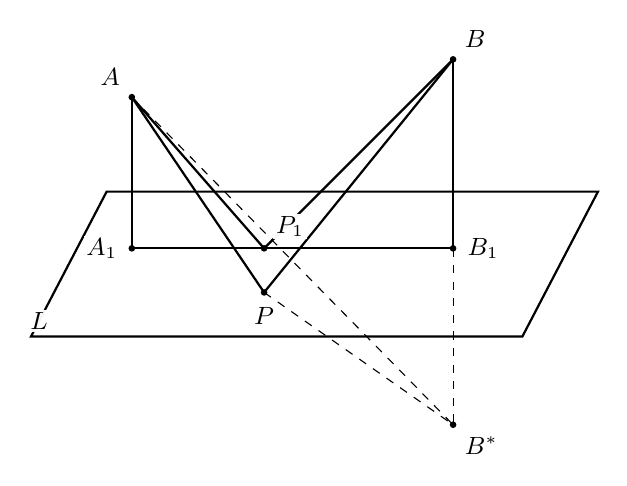
\begin{tikzpicture}[x=0.8cm,y=0.8cm,>=stealth,every node/.style={font=\small,fill=white,fill opacity=.96,text opacity=1,inner sep=1pt,outer sep=1.3pt}]
  \coordinate (A1) at (1.6,1.65);
  \coordinate (B1) at (6.7,1.65);
  \coordinate (A) at (1.6,4.05);
  \coordinate (B) at (6.7,4.65);
  \coordinate (Bs) at (6.7,-1.15);
  \coordinate (P) at (3.7,0.95);
  \coordinate (P1) at (3.7,1.65);
  \draw[thick] (0.0,0.25)--(7.8,0.25)--(9.0,2.55)--(1.2,2.55)--cycle;
  \node[left=3pt] at (0.5,0.5) {$L$};
  \draw[thick] (A1)--(B1);
  \draw[thick] (A1)--(A);
  \draw[thick] (B1)--(B);
  \draw[dashed] (B1)--(Bs);
  \draw[thick] (A)--(P)--(B);
  \draw[thick] (A)--(P1)--(B);
  \draw[dashed] (A)--(Bs);
  \draw[dashed] (P)--(Bs);
  \fill (A) circle (1.2pt) node[above left=2pt] {$A$};
  \fill (A1) circle (1.2pt) node[left=3pt] {$A_1$};
  \fill (B) circle (1.2pt) node[above right=2pt] {$B$};
  \fill (B1) circle (1.2pt) node[right=3pt] {$B_1$};
  \fill (Bs) circle (1.2pt) node[below right=2pt] {$B^{*}$};
  \fill (P) circle (1.2pt) node[below=3pt] {$P$};
  \fill (P1) circle (1.2pt) node[above right=2pt] {$P_1$};
\end{tikzpicture}
\caption*{图3-1-2}
\end{figure}

下面再举一个光学中的例子，光学在17世纪也是一个重要的科学分支，这当然是与望远镜和显微镜的发明分不开的。而特别是望远镜，是天文研究最有力的工具。于是几何光学兴起了（波动光学则晚到19世纪才流行起来），而17--18世纪的几乎所有大数学家、大物理学家（包括牛顿）对光学都作出了贡献。我们特别要举出费马（Pierre de Fermat，1601--1665）。他其实也是微积分学的奠基者之一。他的方法如下：例如，要考虑光的反射问题，设 $L$ 是一个平面镜面，光线从 $A$ 点射向 $L$ 并在点 $P$ 反射到 $B$ 点，问反射点 $P$ 的位置是什么？当费马着手解决这个问题时，他已经有了一个著名的费马原理：光在一切可能的路径中必取耗时最短的路径。这里要注意什么是“可能的路径”？即联结 $A$ 与 $L$ 上一点 $P$ 再到 $B$ 的路径，如果找到了这样一条路径，$AP$ 必为直线，因为在镜面以外，光当然也走耗时最短因此长度也最短的路径——直线，同理 $PB$ 也是直线。我们可以看到，若由 $A,B$ 两点作 $L$ 之垂线，令垂足为 $A_1,B_1$，则 $AA_1$ 与 $BB_1$ 决定一个与 $L$ 垂直的平面 $M$，$P$ 必在此平面上（图3-1-2）。不然的话，由 $P$ 向此平面 $M$ 作垂线，令垂足为 $P_1$，则 $AP>AP_1$，同理 $BP>BP_1$。从而 $AP+PB>AP_1+P_1B$，而 $APB$ 这条路径就不会是最短路径了。这样，问题就化成了平面问题：在平面 $M$ 上有一直线 $L$ 与线外同侧两点 $A$ 与 $B$，在 $L$ 上求一点 $P_1$ 使 $AP_1+P_1B$ 达到最小值。

用对称点的方法求解这个问题是读者们熟知的，这个方法可以追溯到古希腊的海伦（Heron，大约生于公元1世纪），但它不能推广到更复杂的问题，所以我们以折射问题为例说明费马的方法。设平面 $M$ 上有一直线 $L$，分 $M$ 为上、下两半，在其中光速分别为 $v_1$ 与 $v_2$，在上、下半平面上各取一点 $A$ 与 $B$，问，若光线由 $A$ 经 $L$ 上某一点 $P$ 折射后能到达 $B$，$P$ 之位置何在（图3-1-3）？我们不妨设 $P$ 之坐标为 $x$，从而光走折线 $APB$ 所需的时间是 $x$ 的函数：
\begin{equation}
 f(x)=\frac{AP}{v_1}+\frac{PB}{v_2}.
 \tag{1}
\end{equation}

\begin{figure}[htbp]
\centering
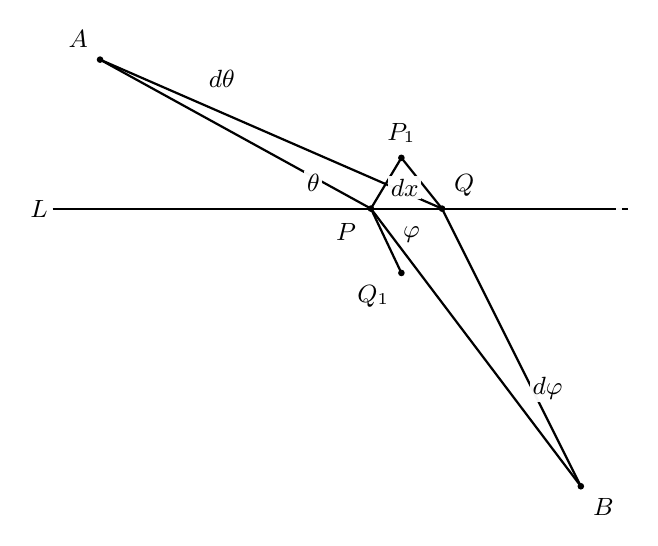
\begin{tikzpicture}[x=0.86cm,y=0.86cm,>=stealth,every node/.style={font=\small,fill=white,fill opacity=.96,text opacity=1,inner sep=1pt,outer sep=1.4pt}]
  \coordinate (A) at (0.3,4.1);
  \coordinate (P) at (4.3,1.9);
  \coordinate (Q) at (5.35,1.9);
  \coordinate (B) at (7.4,-2.2);
  \coordinate (P1) at (4.75,2.65);
  \coordinate (Q1) at (4.75,0.95);
  \draw[thick] (-0.4,1.9)--(8.1,1.9) node[left=1pt] {};
  \node[left=3pt] at (-0.25,1.9) {$L$};
  \draw[thick] (A)--(P)--(B);
  \draw[thick] (A)--(Q)--(B);
  \draw[thick] (P)--(P1);
  \draw[thick] (P)--(Q1);
  \draw[thick] (P1)--(Q);
  \fill (A) circle (1.2pt) node[above left=2pt] {$A$};
  \fill (P) circle (1.2pt) node[below left=3pt] {$P$};
  \fill (Q) circle (1.2pt) node[above right=2pt] {$Q$};
  \fill (B) circle (1.2pt) node[below right=2pt] {$B$};
  \fill (P1) circle (1.2pt) node[above=3pt] {$P_1$};
  \fill (Q1) circle (1.2pt) node[below left=2pt] {$Q_1$};
  \node[above=2pt] at (4.80,1.9) {$dx$};
  \node at (3.45,2.28) {$\theta$};
  \node at (4.9,1.52) {$\varphi$};
  \node[above=1pt] at (2.1,3.55) {$d\theta$};
  \node[right=1pt] at (6.55,-0.75) {$d\varphi$};
\end{tikzpicture}
\caption*{图3-1-3}
\end{figure}

费马的想法是，让 $x$ 变动一个“无穷小量” $dx$ 到 $Q$，$Q$ 的坐标是 $x+dx$（费马当时用 $E$ 或 $e$ 来记 $dx$），于是所需时间成为
\[
f(x+dx)=\frac{AQ}{v_1}+\frac{QB}{v_2}.
\]
比较 $f(x+dx)$ 与 $f(x)$。如果 $f$ 在 $x$ 点达到极小，则当向右移动（$dx>0$）时，$f(x+dx)-f(x)\ge0$，就表示 $f(x)$ 不会再有下降的可能；当 $x$ 向左移动（$dx<0$）时，则又有 $f(x+dx)-f(x)\ge0$，就表示 $f(x)$ 不会比 $f(x+dx)$ 更大了。同样，若 $dx>0$ 时，$f(x+dx)-f(x)<0$，$dx<0$ 时，$f(x+dx)-f(x)<0$，也表明 $f(x)$ 不是极小。因此，要使 $f(x)$ 为极小，$f(x+dx)-f(x)$ 不论 $dx$ 符号如何，总是非负的。我们就来计算 $f(x+dx)-f(x)$，具体说来就是要计算 $(AQ-AP)+(BQ-BP)$，至此，一切都是显然的。费马的“诀窍”就在于计算 $AQ-AP$ 时略去了“应该略去”的东西。过 $P$ 点作 $AQ$ 之垂线 $PP_1$，如果 $dx$ 是无穷小，则由正弦定理，$d\theta$ 也是同阶的“无穷小”（注意，我们这里使用了现代的语言，在费马时代，人们还为无穷小量是不是不可分量等等纠缠不清）所以
\[
AP_1=AP\cos(d\theta)=AP
\]
（其中最多相差一个高阶无穷小量，用费马的记号，则是相差一个 $E^2$ 差不多的东西，在费马看来，这个差不多的东西正是“应该略去的”东西。）因此
\[
AQ-AP=P_1Q=PQ\cos(\theta-d\theta)=dx\cdot\cos\theta.
\]
同理
\[
QB-PB=-PQ_1=-PQ\cos\varphi=-dx\cdot\cos\varphi.
\]
这样
\[
f(x+dx)-f(x)=\left[\frac{\cos\theta}{v_1}-\frac{\cos\varphi}{v_2}\right]dx.
\]
这里最多相差一个高阶无穷小，用费马的记号是相差一个 $E^2$ 的同类项。上式双方除以 $dx$ 即除以 $E$，令 $dx\to0$（费马本人就干脆说令 $E=0$）则费马推出，折射点的位置 $P$ 应适合
\[
\frac{\cos\theta}{v_1}=\frac{\cos\varphi}{v_2}.
\]
只有这样才能适合 $x$ 点即 $P$ 点为极小的条件。但在光学文献中我们通常用光线与 $P$ 点处的法线的夹角而不是与 $L$ 的夹角来表示其方向。故 $\theta=\dfrac{\pi}{2}-\theta_i$（$\theta_i$ 称为入射角），$\varphi=\dfrac{\pi}{2}-\theta_r$（$\theta_r$ 称为折射角），就得到折射点的位置是
\[
\frac{\sin\theta_i}{v_1}=\frac{\sin\theta_r}{v_2}.
\]
在物理学中这叫做斯涅耳（Willibrord Snell）定律。其实笛卡儿也得到了这个定律，而且费马解决了希腊时代托勒密未能解决的问题。

用我们今天的语言来说，即令 $dx\to0$ 而求极限，并令其为0：
\[
\lim_{dx\to0}\frac{f(x+dx)-f(x)}{dx}=f'(x)=
\left[\frac{\sin\theta_i}{v_1}-\frac{\sin\theta_r}{v_2}\right]=0.
\]
但是在费马的时代人们还在为无穷小量是什么而困扰：费马说 $E$ 是无穷小量，那么它究竟是不是0？如果是0，那么从一开始我们就停在 $P$ 点，而不会前进到 $Q$ 点，因此整个讨论就都无法进行了；如果不是0，为什么在经过许多计算后，在关键的一步上说“令 $E=0$”？有了我们今天对无穷小量的理解，我们知道，无穷小量并不是“不可分量”，而是趋于0的变量；并不是“令 $E=0$”，而是令 $dx\to0$。高阶的无穷小量在除以 $dx$ 后，仍会趋向0。所以我们说是：丢掉高阶无穷小量。

以上我们通过实例说明了微分学的基本思想就是“丢掉高阶无穷小”。要注意，当时的大数学家、大数学物理学家，不但是在某种社会经济发展和科学探索的需要的推动下工作，而且是在一定的文化、科学的传统下工作。从欧几里得以来，数学的严格性、合理性的要求，并不如常人认为的那样是一种过分的苛求。牛顿写《原理》以《几何原本》为范本，就是这种表现。那么，什么是无穷小，它是不是零，诸如此类的问题自然成了他的最放心不下心的事。所以，一方面牛顿自称“在数学中最微小的误差也不可以忽略”，另一方面，反对他的人就以此相讥：“高阶无穷小何以可以略去？”——一直到19世纪中晚期，这场大争论才尘埃落定，微积分学才站在稳固的基础上，就是我们今天的教材的讲法，而略去高阶无穷小这个威力强大的方法也就得了无疑问的公认了。

\medskip
\noindent\textbf{2. 这个基本思想在数学物理中的展开}\quad
自牛顿以后，这场争论如火如荼地进行了两百年。可是人们并不只是坐而论道，而是把牛顿的这个思想用于各个方面。因为牛顿既然对机械运动提出了一个包罗万象的理论，而且公认是人类思想史上对认识大自然的第一次伟大的综合（综合就是总结），人们当然就会把它用于机械运动的各个方面：流体、弹性体、声学……都纳入了科学家的视野，成了新生的数学武器——微积分学——的试验场。下面我们将要介绍“略去高阶无穷小”这个基本方法怎样帮助我们得到某些领域的基本规律的数学表述。但是这些规律的物理内容都比较简单，大体上都是例如质量守恒、动量守恒等等，因此都是牛顿力学的适用范围。

第一个例子是热传导方程。热现象本来在牛顿力学的视野之外。人们认真地研究热现象是19世纪的事。那时有了热力学，能量守恒定律内容的丰富性才开始展现。然后是统计物理，使统计的、随机的观点进入了物理学。因此，研究热现象应该从这个观点着眼。但是下面介绍的研究的出发点却是把热当作一种“流体”——热质说。从物理上说，它是很不够的，但是从数学上说却简单得多，而且带来了料想不及的丰硕成果。至于从概率的观点来描述热传导以至得出同样的方程，在第四章 §4 将简单介绍。

1811年巴黎科学院悬赏解决以下问题：“给出热的传播规律数学理论，并将理论结果与精密的实验结果相比较。”应征得奖者是傅里叶（Jean-Baptiste Joseph Fourier，1768--1830）。后来他把自己关于这方面的结果写成一本书，即《热的解析理论》（\textit{Théorie Analytique de la Chaleur}，中文译本，武汉出版社1993年出版）。这是一篇伟大的著作。人们认为傅里叶的功绩有两个方面，首先他把物理问题用线性偏微分方程来表示，使得牛顿在《原理》一书中开创的道路远远扩展到了《原理》一书所规定的范围之外；其次，他为解决这些物理问题创造了一种数学理论，开创了“调和分析”理论，至今约二百年，长盛不衰，始终是数学主流的一部分。这在数学史上是少见的。本书将在第五章相当详尽地加以介绍。

\begin{figure}[htbp]
\centering
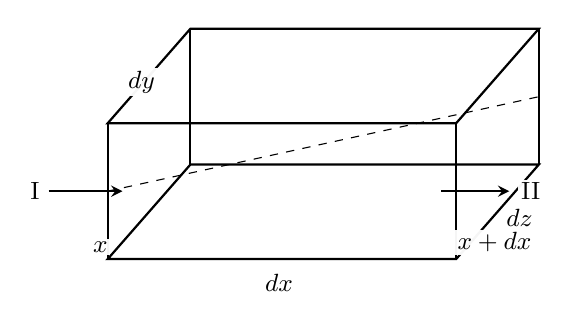
\begin{tikzpicture}[x=0.75cm,y=0.75cm,>=stealth,every node/.style={font=\small,fill=white,fill opacity=.96,text opacity=1,inner sep=1pt,outer sep=1.3pt}]
  \coordinate (A) at (0,0);
  \coordinate (B) at (5.9,0);
  \coordinate (C) at (7.3,1.6);
  \coordinate (D) at (1.4,1.6);
  \coordinate (At) at (0,2.3);
  \coordinate (Bt) at (5.9,2.3);
  \coordinate (Ct) at (7.3,3.9);
  \coordinate (Dt) at (1.4,3.9);
  \draw[thick] (A)--(B)--(C)--(D)--cycle;
  \draw[thick] (At)--(Bt)--(Ct)--(Dt)--cycle;
  \draw[thick] (A)--(At) (B)--(Bt) (C)--(Ct) (D)--(Dt);
  \draw[dashed] (0,1.15)--(7.3,2.75);
  \draw[->,thick] (-1.0,1.15)--(0.25,1.15);
  \draw[->,thick] (5.65,1.15)--(6.8,1.15);
  \node[left=2pt] at (-0.95,1.15) {I};
  \node[right=2pt] at (6.8,1.15) {II};
  \node[below=3pt] at (2.9,0) {$dx$};
  \node[below=3pt] at (6.55,0.7) {$x+dx$};
  \node[left=2pt] at (0.2,0.2) {$x$};
  \node[left=2pt] at (1.0,3.0) {$dy$};
  \node[right=2pt] at (6.55,0.7) {$dz$};
\end{tikzpicture}
\caption*{图3-1-4}
\end{figure}

为简单起见，在热传导的区域中切出一块无穷小的长方体，其棱平行于坐标轴，而三边长度分别是无穷小 $dx,dy,dz$。设热量通过其各个面进入这个无穷小区域（注意，关于热本质的了解要等到19世纪后半叶，而在傅里叶的时代，人们仍把热看成一种流体——热质，傅里叶的著作中仍沿袭了这个观点），如果我们记 $(x,y,z)$ 处时刻 $t$ 的温度为 $u(x,y,z,t)$，则例如图3-1-4断面 I 处，依外法线方向（现在外法线方向即 $-x$ 方向）在时刻 $t$ 到 $t+dt$ 之间流入区域的“热量”应与温度的梯度、断面 I 的面积以及时段长度成正比，因此应为
\begin{equation}
 k\,dy\,dz\,dt\,\frac{\partial u(x,y,z,t)}{\partial n}
 =-k\,dy\,dz\,dt\,\frac{\partial u(x,y,z,t)}{\partial x}.
 \tag{2}
\end{equation}
$k$ 是一个比例常数，称为传导系数，一般说来，$k$ 是 $(x,y,z)$ 的函数，是表征介质的传热性质的，现在为简单起见设它是常数。注意这里我们用了一个点 $(x,y,z)$ 一个时刻 $t$ 的温度状况来表示一个断面、一段时间的温度状况，自然就会有误差，但由于断面面积 $dy\,dz$ 以及时段长度 $dt$ 均为无穷小，所以误差应为高阶无穷小，按我们上面的规定：高阶无穷小可以略去不计，这样才得到(2)式。用同样的方法处理断面 II，不过注意，这时外法线方向即 $x$ 方向，从而 $\dfrac{\partial u}{\partial n}=\dfrac{\partial u}{\partial x}$，由前所述知，经过断面 II 在时刻 $t$ 到 $t+dt$ 之间流入该无穷小区域的热量应是
\begin{equation}
 k\,dy\,dz\,dt\,\frac{\partial u(x+dx,y,z,t)}{\partial x}.
 \tag{3}
\end{equation}
(2)、(3)之和是
\begin{equation}
 k\left[\frac{\partial u(x+dx,y,z,t)}{\partial x}-\frac{\partial u(x,y,z,t)}{\partial x}\right]dy\,dz\,dt
 =k\left[\frac{\partial^2u(x,y,z,t)}{\partial x^2}dx\right]dy\,dz\,dt.
 \tag{4}
\end{equation}
注意，在利用拉格朗日公式时，我们又略去了一个高阶无穷小量。至此，$x$ 方向的热流已经清楚了。用完全同样的方法处理 $y,z$ 方向的热流，我们将得到，在 $t$ 到 $t+dt$ 之间经过该无穷小区域之表面进入的热量总量是
\begin{equation}
 dQ=k\left(\frac{\partial^2u}{\partial x^2}+\frac{\partial^2u}{\partial y^2}+\frac{\partial^2u}{\partial z^2}\right)dx\,dy\,dz\,dt
 =k\Delta u(x,y,z,t)dx\,dy\,dz\,dt.
 \tag{5}
\end{equation}
这里我们引入了一个记号 $\Delta$，我们称它为拉普拉斯算子：
\[
\Delta=\frac{\partial^2}{\partial x^2}+\frac{\partial^2}{\partial y^2}+\frac{\partial^2}{\partial z^2}.
\]
它可能是数学物理中“最重要的”算子了。它的形状如此简单是否隐含了大自然的某种奥秘？是的，它表现了空间（爱因斯坦以前的空间）是均匀和各向同性的。我们暂置不论，倒是 $dQ$ 的流入将导致温度的改变，即由 $u(x,y,z,t)$ 变成 $u(x,y,z,t+dt)$，温差是
\[
u(x,y,z,t+dt)-u(x,y,z,t)\approx \frac{\partial u}{\partial t}dt.
\]
这里我们又略去了高阶无穷小。可是使单位质量的介质温度上升所需的热量应与质量以及温度增量成正比，比例常数 $c$ 称为比热。现在该无穷小区域的介质之质量是 $\rho\,dx\,dy\,dz$（$\rho$ 是密度），所以又应有
\begin{equation}
 dQ=c\rho\frac{\partial u}{\partial t}dt\,dx\,dy\,dz.
 \tag{6}
\end{equation}
比较(5)和(6)，立即得到温度 $u$ 所应适合的方程
\begin{equation}
 \Delta u=\frac{c\rho}{k}\frac{\partial u}{\partial t}=\frac1{a^2}\frac{\partial u}{\partial t},\qquad a^2=\frac{k}{c\rho}.
 \tag{7}
\end{equation}
这里我们又假设了 $c,\rho$ 都是常数。

方程(7)称为热传导方程。可是值得注意的是，不仅是热传导现象由它来描述，而且扩散现象，渗流，化学反应乃至生物的繁殖与迁移等等也都是由它或由它衍生的方程来反映。数学物理中的偏微分方程大多有此特点。例如，波动方程不但能反映声波，而且也能刻画电磁波，以及一定条件下的水波、空气中的波等等，定常现象则常用拉普拉斯方程
\begin{equation}
 \Delta u=\frac{\partial^2u}{\partial x^2}+\frac{\partial^2u}{\partial y^2}+\frac{\partial^2u}{\partial z^2}=0
 \tag{8}
\end{equation}
来刻画。静电场的势，引力场的势等等都适合这样的方程。

现在应特别注意以下的事实，(7)是一个很一般的方程，即是说，只要传热的物体 $\Omega$ 是均匀的，因此 $c$ 和 $k$ 都是常数，密度 $\rho$ 也是常数，则不论该物体是什么形状，处于什么条件下，总是这一个方程。因此，在解决具体问题时，总要附加一些条件。一是应该知道在初始时刻（设为 $t=0$）该物体内的温度分布，这样就有了一个附加条件
\begin{equation}
 \left.u\right|_{t=0}=\varphi(x,y,z),\qquad (x,y,z)\in\Omega.
 \tag{9}
\end{equation}
$\varphi(x,y,z)$ 是已知函数。(9)称为初始条件。二是 $\Omega$ 边界上 $\partial\Omega$ 的情况也很重要。这里可以有多种情况，例如知道在 $\partial\Omega$ 上的温度分布，这时有
\begin{equation}
 \left.u\right|_{\partial\Omega}=\psi(x,y,z),\qquad (x,y,z)\in\partial\Omega,
 \tag{$10_1$}
\end{equation}
另一种情况是假设 $\Omega$ 与外界没有热交换——绝热情况，则有
\begin{equation}
 \left.\frac{\partial u}{\partial n}\right|_{\partial\Omega}=0,
 \tag{$10_2$}
\end{equation}
$n$ 是 $\partial\Omega$ 的法线方向。还可能有其它情况。(10$_1$)与(10$_2$)中只需限定一个就可以了，这称为边值条件。至于一个方程应该附加什么样的条件，在有了这些附加条件下是否有解存在，是否只有一个解，这个解（或这些解）有什么性质，又如何求法，这些都是严重问题。我们现在只想指出：一方面有一个方程（如(8)那样）来刻画一般的物理规律，另一方面又有一些附加条件，反映具体问题的具体情况，这是牛顿的伟大创造，并不是说牛顿给出了初始条件、边值条件这些名词和概念，而是从他开始就这样研究问题了。

第二个例子是关于流体的动力学。我们把流体看作连续介质（在一些极端情况下就不能这样看，例如在大气层上层空气极端稀薄处，就需要把气体看成随机运动、碰撞的分子的集合，这时就不能采用连续介质的模型。但是在牛顿的时代以及后来的18--19世纪当然不是这样）。这样一来，流体力学就成了牛顿力学的延伸。在这个模型下研究流体的基本方法是：在流体中切出无穷小一块，视作一个质点。然后考虑质量守恒、动量守恒即可。为什么不说能量守恒？因为要讨论流体（特别是气体）中的能量守恒，就至少要加上热力学的考虑。这样一来，关于内能，熵……会出现一大堆新问题。流体力学对于空气中的飞行，如飞机、导弹等等，当然是极其重要的。到了20世纪中叶，例如由于飞机速度越来越高，这些热力学考虑是不可避免的。在更高速度情况下，还要考虑电磁场的影响，化学反应的影响等等。但是在18--19世纪，还可以只限于机械能的考虑。例如对船舶在水中航行，通常都把水看成不可压缩流体，这样只考虑机械能就够了。不过即使在这时，对流体的基本性质也要加上限制。我们的限制是只考虑理想流体。研究各种流体都少不了研究其速度场：$\boldsymbol u(x,y,z,t)=(u_1,u_2,u_3)$，这是一个依赖于 $(x,y,z,t)$ 的向量场，还有密度 $\rho(x,y,z,t)$ 以及压强 $p(x,y,z,t)$。（因为我们有意忽略热力学的考虑，所以也略去了温度 $T(x,y,z,t)$ 的研究）。压强就是单位面积上所受的压力，它本应是有方向的量（有方向的量不只是向量，还有张量，这一点详见第七章）。但我们现在取 $p=p(x,y,z,t)$ 为一标量，其原因就在于我们只考虑理想流体。理想流体就是没有黏性，又不必考虑热传导的流体。如果我们在流体内作一截面 $S$，则在紧邻接着 $S$ 的 $P(x,y,z)$ 点，其一侧 I 的流体必向另一侧 II 的流体施压力（图3-1-5）。这个压力还依赖于 $S$ 的方向（不妨设为由 II 伸向 I 的法线 $\boldsymbol n$ 方向），所以压力包含了两个方向要素。在数学上我们用张量来描述它。所谓理想流体就是不论取什么样的截面 $S$，压力方向总在上述法线方向 $\boldsymbol n$ 上，其大小也不随 $\boldsymbol n$ 改变。这就是没有黏性作用的表现。单位面积上的压力称为压强。所以在理想流体中，由 I 向 II 施加的压力应为
\[
p(x,y,z,t)\cdot S\text{ 之面积}\cdot\boldsymbol n.
\]
所以刻画理想流体各部分相互作用的内力，只需要一个标量函数 $p=p(x,y,z,t)$ 就够了。这就是规定压强为标量函数的原因。

\begin{figure}[htbp]
\centering
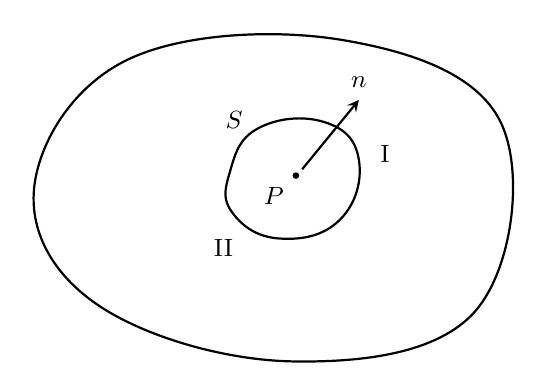
\begin{tikzpicture}[x=0.8cm,y=0.8cm,>=stealth,every node/.style={font=\small,fill=white,fill opacity=.96,text opacity=1,inner sep=1pt,outer sep=1.4pt}]
  \draw[thick] plot[smooth cycle,tension=.65] coordinates {(-3.7,0.2) (-2.2,2.2) (1.2,2.5) (3.7,1.2) (3.3,-1.8) (0.4,-2.6) (-2.7,-1.7)};
  \draw[thick] plot[smooth cycle,tension=.75] coordinates {(-0.6,0.4) (-0.15,1.1) (0.9,1.2) (1.45,0.6) (1.15,-0.35) (0.2,-0.65) (-0.55,-0.25)};
  \fill (0.45,0.35) circle (1.2pt) node[below left=2pt] {$P$};
  \node[above left=2pt] at (-0.2,0.9) {$S$};
  \draw[->,thick] (0.55,0.45)--(1.45,1.55) node[above=2pt] {$\boldsymbol n$};
  \node[right=2pt] at (1.6,0.7) {I};
  \node at (-0.7,-0.8) {II};
\end{tikzpicture}
\caption*{图3-1-5}
\end{figure}

现在在理想流体内切出其棱平行于坐标轴的无穷小块，其三边之长分别是无穷小量 $dx,dy,dz$。我们先讨论质量守恒。在 $(t,t+dt)$ 时间段内从外面流入这个无穷小块的流体，可以分别由经过 I、II……诸界面的流体计算得出（图3-1-6）。例如经过 I 的流体将成为一个边长为 $u_1dt$ 而断面面积为 $dy\,dz$ 的柱子，因此，其质量为
\[
(\rho u_1)(x,y,z,t)dt\,dy\,dz.
\]
同样，经过 II 流入的流体质量是 $-(\rho u_1)(x+dx,y,z,t)dt\,dy\,dz$，所以由 $x$ 轴方向进入的流体总量是
\[
-\frac{\partial}{\partial x}[\rho u_1(x,y,z,t)]dx\,dy\,dz\,dt.
\]
而由全部边界进入的流体总量是
\[
dQ=-\left[\frac{\partial}{\partial x}(\rho u_1)+\frac{\partial}{\partial y}(\rho u_2)+\frac{\partial}{\partial z}(\rho u_3)\right](x,y,z,t)dt\,dx\,dy\,dz.
\]
这些流体的进入将使该无穷小块中的密度由 $\rho(x,y,z,t)$ 变成 $\rho(x,y,z,t+dt)$，密度的增加所占用的流量就是 $dQ$，故在略去高阶无穷小后
\[
dQ=[\rho(x,y,z,t+dt)-\rho(x,y,z,t)]dx\,dy\,dz
=\frac{\partial\rho}{\partial t}(x,y,z,t)dt\,dx\,dy\,dz.
\]
比较二式即得表征质量守恒的连续性方程：
\begin{equation}
\frac{\partial\rho}{\partial t}+\frac{\partial}{\partial x}(\rho u_1)+\frac{\partial}{\partial y}(\rho u_2)+\frac{\partial}{\partial z}(\rho u_3)
=\frac{\partial\rho}{\partial t}+\operatorname{div}(\rho\boldsymbol u)=0.
\tag{10}
\end{equation}

\begin{figure}[htbp]
\centering
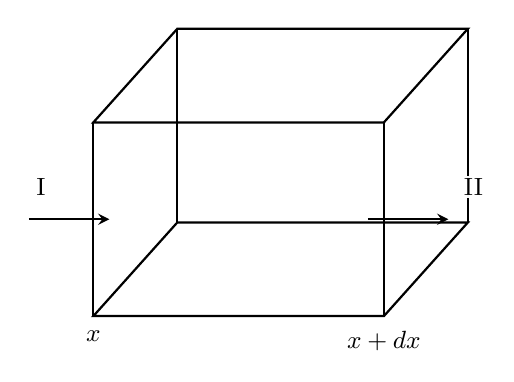
\begin{tikzpicture}[x=0.82cm,y=0.82cm,>=stealth,every node/.style={font=\small,fill=white,fill opacity=.96,text opacity=1,inner sep=1pt,outer sep=1.4pt}]
  \coordinate (A) at (0,0); \coordinate (B) at (4.5,0); \coordinate (C) at (5.8,1.45); \coordinate (D) at (1.3,1.45);
  \coordinate (At) at (0,3.0); \coordinate (Bt) at (4.5,3.0); \coordinate (Ct) at (5.8,4.45); \coordinate (Dt) at (1.3,4.45);
  \draw[thick] (A)--(B)--(C)--(D)--cycle;
  \draw[thick] (At)--(Bt)--(Ct)--(Dt)--cycle;
  \draw[thick] (A)--(At) (B)--(Bt) (C)--(Ct) (D)--(Dt);
  \draw[dashed] (D)--(C);
  \draw[->,thick] (-1.0,1.5)--(0.25,1.5);
  \draw[->,thick] (4.25,1.5)--(5.5,1.5);
  \node[left=2pt] at (-0.55,2.0) {I};
  \node[right=2pt] at (5.55,2.0) {II};
  \node[below=3pt] at (0.0,0) {$x$};
  \node[below=3pt] at (4.5,0) {$x+dx$};
\end{tikzpicture}
\caption*{图3-1-6}
\end{figure}

再看动量守恒，我们也可以引入所谓动量密度流的概念，但这就涉及速度向量的张量积的概念，我们暂不假设读者都知道它，也不打算现在就花很大篇幅去讲解它（第七章中会讲到这里涉及的张量积），因此就直截了当地把这个无穷小流体小块当成一个质点，其质量是 $\rho(x,y,z,t)dx\,dy\,dz$，其速度为 $\boldsymbol u(x,y,z,t)$，然后直接应用牛顿第二定律。其实这里已经包括了舍去高阶无穷小量的思想。例如，一个无穷小元并不真正是一个点，因而其内部不一定是均匀的。我们以 $(x,y,z,t)$ 处的密度作为此无穷小元内各点 $t$ 时的密度，本身就有一个误差，只不过这样算出的质量与真正的质量也就只差一个高阶无穷小。下面计算加速度和外力时也都如此。

在计算加速度时要注意，速度 $\boldsymbol u(x,y,z,t)$ 中的 $x,y,z$ 都是 $t$ 的函数，$x=x(t),y=y(t),z=z(t)$ 即该质点的轨迹，所以在计算 $\dfrac{d\boldsymbol u}{dt}$ 时，既要看到第四个变元 $t$ 在变化而 $x,y,z$ 不变时产生的加速度 $\dfrac{\partial\boldsymbol u}{\partial t}$（称为当地加速度），又要看到因为 $(x,y,z)$ 随着时间变化而改变位置使 $\boldsymbol u$ 也得到一个加速度
\[
\frac{\partial\boldsymbol u}{\partial x}\frac{dx}{dt}+\frac{\partial\boldsymbol u}{\partial y}\frac{dy}{dt}+\frac{\partial\boldsymbol u}{\partial z}\frac{dz}{dt}
=u_1\frac{\partial\boldsymbol u}{\partial x}+u_2\frac{\partial\boldsymbol u}{\partial y}+u_3\frac{\partial\boldsymbol u}{\partial z}
=\left(u_1\frac{\partial}{\partial x}+u_2\frac{\partial}{\partial y}+u_3\frac{\partial}{\partial z}\right)\boldsymbol u
\]
（称为对流加速度），所以
\begin{equation}
\begin{aligned}
\frac{d\boldsymbol u}{dt}
&=\text{当地加速度}+\text{对流加速度}\\
&=\frac{\partial\boldsymbol u}{\partial t}
 +\left(u_1\frac{\partial}{\partial x}+u_2\frac{\partial}{\partial y}+u_3\frac{\partial}{\partial z}\right)\boldsymbol u\\
&=\frac{\partial\boldsymbol u}{\partial t}+(\boldsymbol u\cdot\operatorname{grad})\boldsymbol u.
\end{aligned}
\tag{11}
\end{equation}

最后看外力，外力有两个部分，一是流体之外来的力，例如重力，又例如当流体是带电的，同时又处在电磁场中的电磁力，这时我们得到了电磁流体力学。还有例如流体中有某种化学反应或燃烧、爆炸而产生的力。我们记这种外力的质量密度（即作用在单位质量上的外力）为 $\boldsymbol F$。第二部分是流体中这个无穷小元以外各部分对它的力，亦即压力，这一部分我们已计算了。例如通过 I、II 两个面的作用力是
\begin{equation}
-p(x+dx,y,z,t)dy\,dz+p(x,y,z,t)dy\,dz=-\frac{\partial p}{\partial x}dx\,dy\,dz.
\tag{12}
\end{equation}
把这些结果综合起来，由牛顿第二定律：
\[
\text{质量}\times\text{加速度}=\text{外力}
\]
有
\[
\rho\,dx\,dy\,dz\frac{d\boldsymbol u}{dt}=\rho\,dx\,dy\,dz\cdot\boldsymbol F-\operatorname{grad}p\,dx\,dy\,dz.
\]
于是我们得到表观动量守恒的方程
\begin{equation}
\frac{d\boldsymbol u}{dt}=\frac{\partial\boldsymbol u}{\partial t}+(\boldsymbol u\cdot\operatorname{grad})\boldsymbol u=-\frac1\rho\operatorname{grad}p+\boldsymbol F.
\tag{13}
\end{equation}
(10)和(13)就是流体力学的基本方程组，如上所述，它们是不完备的，因为热力学的考虑都被忽略了。它是一个极广泛又极困难的领域的起点。

\enlargethispage{1.5\baselineskip}
以上我们通过两个例子表明，应用微分学的基本思想于研究自然界的许多广泛领域，得到了描述其基本物理规律的微分方程（这两个例子都是偏微分方程（PDE），下面我们将见到常微分方程（ODE）的例子）。微分方程是数学中范围极广泛、内容极丰富而且又极困难的领域，在许多自然科学分支中，它是基本的数学工具。我们可能以为略去高阶无穷小是产生这些微分方程的最重要的方法。实际上，这是由于我们现在研究的物理过程都比较简单，因而一些守恒律都变得很简单。随着科学的发展，我们需要解决的问题更深刻，所应用的数学工具也更深刻，这时，单只是“略去高阶无穷小”的方法就很不够了。我们将在本书最后介绍麦克斯韦方程组，以便了解数学的发展怎样帮助我们在更深的层次上认识自然界。

\medskip
\noindent\textbf{3. 牛顿与开普勒}\quad
牛顿写的《原理》是为了研究物体的运动，而所谓物体，上至日月星辰，下至苹果树上落下的苹果，无所不包。这样才看出《原理》是认识大自然的规律性的第一次伟大的综合。但是牛顿的三定律中讲的“物体”，其实是指的质点。例如第一定律，牛顿的陈述原文如下：“每个物体都保持其静止、或匀速直线运动的状态，除非有外力作用于它迫使它改变那个状态”。（《原理》中译本，13页）。然而牛顿紧接着举的例子却有陀螺，并指出陀螺各个部分的“凝聚力不断使之偏离直线运动，如果没有空气的阻碍，就不会停止旋转。”可见，如果不是质点而是有内部构造，分成各部分的物体，如陀螺，牛顿也承认，其运动并不一定是匀速直线运动，而可以是旋转。把物体当成质点无非两个办法：一是如果空间极大，则哪怕是日月星辰，在浩瀚无垠的太空中也只是一沧海一粟的质点而已；二是物体有各部分，则各个部分若取得足够小，如上面两个例子中讲的无穷小的一块，小到对其内部结构，对其内部的不均匀性等等都可以忽略不计时，则其各部分也就看成一个质点，而物体整体则看成一个质点组。当然质点组中的质点总数可以是有限的，例如研究地球受太阳、月亮的作用而运动时，我们只需考虑由日、月、地三个质点形成的质点组，而其它行星和火星等等的影响都暂不考虑了，这就是著名的三体问题。这样，由牛顿的第二定律可以得出
\begin{equation}
 m_i\frac{d^2x_i}{dt^2}=f_i\left(t,x,\frac{dx}{dt}\right),\quad i=1,\ldots,N.
 \tag{14}
\end{equation}
注意，这里的 $N$ 不一定是质点的个数。因为每一个质点可以有三个坐标，即相应于三个 $x_i(t)$。

牛顿遇到的问题通常并不是已知 $x_1(t),\ldots,x_N(t)$ 然后求它们的二阶导数，而通常是已知 $f_i\left(t,x,\dfrac{dx}{dt}\right)$，要求未知的 $x_i(t)$，这就是求解作为一个常微分方程（ODE）组的(14)。正如前一段所说的，应该加上某些附加条件。从物理上看，只要知道这个质点组内各质点在初始时刻（例如可设为 $t=0$）的位置及速度就足以完全确定这个质点组在以后的运动状况。因此，我们所需的附加条件是
\begin{equation}
 x_i(0)=x_i^0,\qquad \frac{dx_i(0)}{dt}=v_i^0.
 \tag{15}
\end{equation}
(15)就是一个初始条件。在一个初始条件下求解(14)，称为一个柯西问题或初值问题（initial value problem）。以上讲的是有限质点组的情况。如果是无穷多个质点所成的质点组，如上面讲的连续介质那样，就会得出偏微分方程组（PDE）。ODE 和 PDE 是两个十分宽阔的数学领域，而且二者由于提出的问题和处理方法不同，又形成很不相似的数学分支。但不论如何，牛顿以后，在18--19世纪中，用数学方法研究大自然的数学规律，几乎就等同于研究微分方程。

牛顿既然已弄清楚了两个物体——质点之间的引力为
\begin{equation}
 \boldsymbol F=-G\frac{m_1m_2}{r^2}\frac{\boldsymbol r}{r},\qquad r=\lVert\boldsymbol r\rVert,
 \tag{16}
\end{equation}
这里设第一个质点（其质量为 $m_1$）位于原点，$\boldsymbol r$ 则是由原点到第二个质点（质量 $m_2$）的向量（如果采用极坐标，$r$ 就是第二个质点的动径），$G$ 是引力常数，则为了求第二个质点的运动方程，只要将(16)代入(14)式并求解这个二阶常微分方程就行了。这个问题称为开普勒问题，或称二体问题。它是由瑞士数学家约翰·伯努利（Johann Bernoulli，1667--1748）\footnote{这里讲的是老约翰·伯努利，有时也称他是约翰·伯努利一世（Johann I. Bernoulli）。他的儿子也叫约翰，所以称为约翰·伯努利二世（Johann II. Bernoulli，1710--1790），也是一位数学家，我们在变分学一节中将介绍他。二世的哥哥丹尼尔·伯努利（Daniel Bernoulli，1700--1782）也是一位大数学家，对流体力学与气体分子运动论、偏微分方程等有大的贡献。至于捷线问题，其实是一世和他的大哥雅各布一世（Jacob I. Bernoulli，1654--1705）开始研究的，雅各布还是概率论的创始人之一。伯努利一家的故事比杨家将其实多了又重要多了。}于1710年最早给出了完整的解答，这已是《原理》以后的23年了。我们看见，现在已不需要再重复“略去高阶无穷小”这个思想，而只要应用在它的基础上建立起来的微积分的种种概念、方法和技巧就行了。鉴于二体问题的解决很好地表明了牛顿的思想的力量，又是科学史上一件大事，我们用现在常见的微积分教材中的方法介绍一下它的解法。

我们记 $k=Gm_1$，并将第二个质点的质量 $m_2$ 就写成 $m$，于是(16)中的 $\boldsymbol F$ 成为
\[
 \boldsymbol F=-\frac{km}{r^2}\frac{\boldsymbol r}{r},
\]
而第二个质点（以下就简称为质点，因为第一个质点已规定静止于原点处，或者说我们以第一个质点为参考系）的运动方程现在成为
\begin{equation}
 \frac{d^2\boldsymbol r}{dt^2}=-\frac{k}{r^2}\frac{\boldsymbol r}{r}.
 \tag{17}
\end{equation}
$\boldsymbol r=(x,y,z)$ 是质点的坐标。为简单起见，我们令 $m=1$，上面的 ODE 组由三个2阶方程组成，相当于6个一阶 ODE。这是一个相当大的方程组。求解的基本思想是降阶，而降阶则通过寻找守恒律来实现。如(17)这样的方程，力 $\boldsymbol F$ 的大小只依赖于 $r$，方向又是 $\boldsymbol r$，这种力称为有心力。我们有

\noindent\textbf{定理1}\quad 质点在有心力作用下运动时，角动量守恒。

\noindent\textbf{证}\quad 一个质点的角动量就是其动量 $m\dot{\boldsymbol r}$（本书遵从牛顿的记号，对时间求导用上加一点来表示）对原点的矩
\[
 \boldsymbol M(t)=m\boldsymbol r(t)\times\dot{\boldsymbol r}(t).
\]
这里“$\times$”表示向量积，不论是标量函数的积，还是标量与向量之积，还是向量之间的标量积、向量积、混合积，求导时都服从莱布尼茨定律。所以
\[
 \dot{\boldsymbol M}(t)=m\dot{\boldsymbol r}\times\dot{\boldsymbol r}+m\boldsymbol r\times\ddot{\boldsymbol r}=0.
\]
第一项等于0是因为 $\dot{\boldsymbol r}$ 与 $\dot{\boldsymbol r}$ 平行，而两个平行向量的向量积一定为0。第二项为0同样是因为 $\ddot{\boldsymbol r}$ 是有心力而与 $\boldsymbol r$ 平行，所以角动量 $\boldsymbol M$ 不随时间改变，定理证毕。

\begin{figure}[htbp]
\centering
\begin{tikzpicture}[x=1.0cm,y=1.0cm,>=stealth,every node/.style={font=\small,fill=white,fill opacity=.96,text opacity=1,inner sep=1pt,outer sep=1.5pt}]
  \coordinate (O) at (0,0);
  \coordinate (P) at (5.0,2.7);
  \draw[->,thick] (-0.2,0)--(6.4,0);
  \draw[->,thick] (O)--(P);
  \draw[->,thick] (3.75,2.02)--(5.25,2.83);
  \draw[->,thick] (4.55,2.46)--(3.75,3.95);
  \draw (1.15,0) arc[start angle=0,end angle=28.4,radius=1.15];
  \node[left=2pt] at (O) {$O$};
  \node[below=2pt] at (2.55,1.38) {$r=|\boldsymbol r|$};
  \node[above=2pt] at (5.25,2.83) {$\boldsymbol e_r$};
  \node[above left=2pt] at (3.75,3.95) {$\boldsymbol e_\varphi$};
  \node[below right=1pt] at (1.00,0.42) {$\varphi$};
  \node[above left=2pt] at (4.35,2.35) {$\boldsymbol r$};
\end{tikzpicture}
\caption*{图3-1-7}
\end{figure}

$\dot{\boldsymbol M}(t)=0$ 不仅表示 $\boldsymbol M(t)$ 大小不变而且方向也不变。这样，$\boldsymbol r$ 与 $\dot{\boldsymbol r}$ 恒在与 $\boldsymbol M$ 正交的平面上。这样一来(17)就变成了平面问题，即 $\boldsymbol r$ 是平面向量，而只有两个分量，不妨设它们就是 $\boldsymbol r(t)=(x(t),y(t))$，于是(17)成了两个二阶 ODE 的方程组，相当于4个一阶 ODE。这就是降阶。

我们还可以应用 $M(t)$ 之大小也不变。既然开普勒问题已经化为平面问题，我们就可以引入极坐标系。于是在每一点 $(r,\varphi)$ 处可以引入两个单位向量 $\boldsymbol e_r$——径向向量与 $\boldsymbol e_\varphi$——横向向量，而且 $(\boldsymbol e_r,\boldsymbol e_\varphi)$ 取为右手系（图3-1-7），而且
\begin{equation}
 \boldsymbol r=r\boldsymbol e_r.
 \tag{18}
\end{equation}
\jiaokan{原文(18)式排作“$\boldsymbol r=r\boldsymbol e_r+\varphi\boldsymbol e_\varphi$”。位置向量在平面极坐标基底中的表示应为 $\boldsymbol r=r\boldsymbol e_r$；原文随后的速度推导也正使用这一表示，今据上下文改正。}
我们想在极坐标系下计算一下速度 $\dot{\boldsymbol r}$。在第二章中讲三角函数时我们就讲过这个结果（但是使用的记号不同，现在在 $\boldsymbol e_r$ 与 $\boldsymbol e_\varphi$ 那时记作 $\boldsymbol e_\rho$ 与 $\boldsymbol e_\theta$），由于其重要性，我们再从角动量守恒角度再来算一次。

因为 $\boldsymbol e_r$ 是单位向量，$\boldsymbol e_r\cdot\boldsymbol e_r=1$。对 $t$ 求导有
\[
 \dot{\boldsymbol e}_r\cdot\boldsymbol e_r+\boldsymbol e_r\cdot\dot{\boldsymbol e}_r=2\boldsymbol e_r\cdot\dot{\boldsymbol e}_r=0.
\]
所以 $\dot{\boldsymbol e}_r$ 与 $\boldsymbol e_r$ 正交而与 $\boldsymbol e_\varphi$ 平行。问题是同向还是反向？但是 $\boldsymbol e_r$ 是绕单位圆旋转，所以 $\dot{\boldsymbol e}_r=\dot\varphi\boldsymbol e_\varphi$，同理 $\dot{\boldsymbol e}_\varphi=-\dot\varphi\boldsymbol e_r$：
\begin{equation}
 \dot{\boldsymbol e}_r=\dot\varphi\boldsymbol e_\varphi,\qquad
 \dot{\boldsymbol e}_\varphi=-\dot\varphi\boldsymbol e_r.
 \tag{19}
\end{equation}
这样，由于 $\boldsymbol r=r\boldsymbol e_r$，我们立即有
\begin{equation}
 \dot{\boldsymbol r}=\dot r\,\boldsymbol e_r+r\dot\varphi\,\boldsymbol e_\varphi.
 \tag{20}
\end{equation}
这就是说，速度向量有两个分量，一是径向的 $\dot r\,\boldsymbol e_r$，另一是横向的 $r\dot\varphi\,\boldsymbol e_\varphi$。利用它来计算角动量，有
\[
 \boldsymbol M(t)=\boldsymbol r\times\dot{\boldsymbol r}
 =r\dot r(\boldsymbol e_r\times\boldsymbol e_r)+r^2\dot\varphi(\boldsymbol e_r\times\boldsymbol e_\varphi)
 =r^2\dot\varphi(\boldsymbol e_r\times\boldsymbol e_\varphi).
\]
因为 $\boldsymbol e_r\times\boldsymbol e_\varphi$ 是 $\boldsymbol M(t)$ 方向的单位向量（这由向量积的定义可知），所以 $\boldsymbol M(t)$ 之“大小”是 $r^2\dot\varphi$（$|\boldsymbol M(t)|\ge0$ 而 $M(t)$ 之“大小”却因 $\dot\varphi$ 可能为负而可能小于0），它是守恒的。

设动径 $r(t)$ 扫过的扇形（以原点为顶点）的面积为 $S(t)$，则由图3-1-8易见
\[
 \Delta S=S(t+\Delta t)-S(t)=\frac12r^2\dot\varphi\,\Delta t+o(1)\Delta t.
\]
所以“面积速度”
\[
 \frac{dS}{dt}=\frac12r^2\dot\varphi=\frac12M(t).
\]
因为角动量不随时间变化，所以面积速度也不变。这就是开普勒第二定律。

\begin{figure}[htbp]
\centering
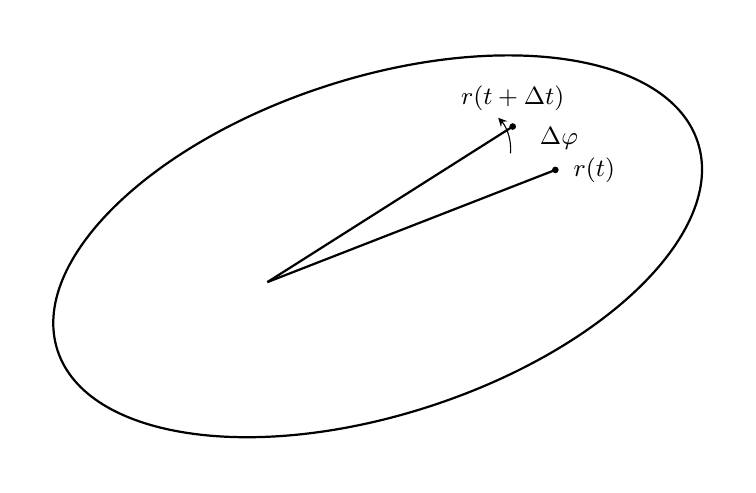
\begin{tikzpicture}[x=0.95cm,y=0.95cm,>=stealth,every node/.style={font=\small,fill=white,fill opacity=.96,text opacity=1,inner sep=1pt,outer sep=1.6pt}]
  \coordinate (F) at (0,0);
  \draw[thick,rotate=18] (1.55,0) ellipse (4.5 and 2.25);
  \coordinate (P) at (3.85,1.50);
  \coordinate (Q) at (3.28,2.08);
  \draw[thick] (F)--(P);
  \draw[thick] (F)--(Q);
  \fill (P) circle (1.2pt);
  \fill (Q) circle (1.2pt);
  \node[right=4pt] at (P) {$\boldsymbol r(t)$};
  \node[above=3pt] at (Q) {$\boldsymbol r(t+\Delta t)$};
  \draw[->] (3.25,1.72) arc[start angle=-5,end angle=43,radius=0.62];
  \node[right=4pt] at (3.40,1.92) {$\Delta\varphi$};
\end{tikzpicture}
\caption*{图3-1-8}
\end{figure}

\noindent\textbf{定理2（开普勒第二定律）}\quad 有心力场中运动的质点恒有不随时间变化的面积速度。这也就是前面讲的第一个例子。

为了看开普勒另外两个定律，我们再来看能量守恒。首先注意，方程(17)中的力是有位能的，其位能是
\[
 U(r)=-\frac{k}{r}.
\]
这是因为牛顿的引力是 $-\operatorname{grad}U(r)$，事实上
\[
 -\frac{k}{r^2}\frac{\boldsymbol r}{r}=-\operatorname{grad}U(r)
 =k\operatorname{grad}\left(\frac1r\right).
\]
但是我们要把(17)这个2维问题化为1维问题，为此我们记住角动量“大小”的守恒值为 $M=r^2\dot\varphi$。由(20)式对 $t$ 再求导，有
\[
 \ddot{\boldsymbol r}=\ddot r\,\boldsymbol e_r+\dot r\dot\varphi\boldsymbol e_\varphi
 +\dot r\dot\varphi\boldsymbol e_\varphi+r\ddot\varphi\boldsymbol e_\varphi+r\dot\varphi\dot{\boldsymbol e}_\varphi
\]
\[
 =\left(\ddot r-r\dot\varphi^2\right)\boldsymbol e_r
 +\left(2\dot r\dot\varphi+r\ddot\varphi\right)\boldsymbol e_\varphi
 =-\operatorname{grad}U(r).
\]
但是
\[
 \operatorname{grad}U(r)=\left(U'(r)\frac{x}{r},U'(r)\frac{y}{r}\right)
 =U'(r)\frac{\boldsymbol r}{r}=U'(r)\boldsymbol e_r,
\]
所以有
\begin{equation}
 \ddot r-r\dot\varphi^2=-U'(r),\qquad 2\dot r\dot\varphi+r\ddot\varphi=0.
 \tag{21}
\end{equation}
以角动量之守恒值代入，得到 $r$ 所适合的方程为
\[
 \ddot r=-\frac{\partial U}{\partial r}+\frac{M^2}{r^3}
 =-\frac{\partial}{\partial r}\left(U+\frac{M^2}{2r^2}\right)
 =-\frac{\partial V}{\partial r}.
\]
这里 $V(r)=U(r)+\dfrac{M^2}{2r^2}$ 称为有效位能。

(21)的后一式没有给我们新信息，因为若用 $r$ 乘此式两边，会得到
\[
 2r\dot r\dot\varphi+r^2\ddot\varphi=\frac{d}{dt}(r^2\dot\varphi)=0,
\]
亦即角动量之“大小”不变。

\noindent\textbf{定理3}\quad 服从(17)的质点的总能量是
\[
 \frac12m\dot{\boldsymbol r}^{\,2}+mU=\frac12m\dot r^{\,2}+mV.
\]
\noindent\textbf{证}\quad 由(20)
\[
 \dot{\boldsymbol r}^{\,2}=\dot{\boldsymbol r}\cdot\dot{\boldsymbol r}
 =\dot r^{\,2}+r^2\dot\varphi^2
 =\dot r^{\,2}+\frac{M^2}{r^2}.
\]
所以
\[
 \frac12\dot{\boldsymbol r}^{\,2}+U
 =\frac12\dot r^{\,2}+\left(U+\frac{M^2}{2r^2}\right)
 =\frac12\dot r^{\,2}+V.
\]
能量守恒和角动量“大小”的守恒就可以用来进一步降阶并求出轨道。事实上，如果令单位质量上的总能量为 $E$（这是一个常数），则由上式有
\[
 \frac{\dot r^{\,2}}2+V=E\quad\text{或}\quad \dot r=\sqrt{2(E-V)}.
\]
又由角动量的大小为 $r^2\dot\varphi=M$，有
\[
 \dot\varphi=M/r^2.
\]
所以
\begin{equation}
 \frac{d\varphi}{dr}=\dot\varphi/\dot r=\frac{M/r^2}{\sqrt{2(E-V)}}.
 \tag{22}
\end{equation}
这样就立刻可以得出

\noindent\textbf{定理4（开普勒第一定律）}\quad 若有心力之位能是 $U(r)=-\dfrac{k}{r}$，则质点运动轨道必为一椭圆，而原点是其一个焦点。

\noindent\textbf{证}\quad 由(22)
\[
 \varphi=\int\frac{M/r^2\,dr}{\sqrt{2(E-V)}}.
\]
以 $V$ 的表达式 $V(r)=U(r)+\dfrac{M^2}{2r^2}=-\dfrac{k}{r}+\dfrac{M^2}{2r^2}$ 代入上式并作积分（需要作一个变量变换 $\rho=\dfrac1r$），立即有
\[
 \varphi=\arccos\frac{\dfrac Mr-\dfrac kM}{\sqrt{2E+\dfrac{k^2}{M^2}}},
\]
或者
\begin{equation}
 r=\frac{p}{1+e\cos\varphi}.
 \tag{23}
\end{equation}
这就是椭圆的极坐标方程，或称焦方程，其中
\[
 p=M^2/k,\qquad e=\sqrt{1+2EM^2/k^2}.
\]
$p$ 称为椭圆的焦半径，$e$ 称为其离心率。它们与长短半轴 $a,b$ 之关系是
\[
 e=\frac ca=\frac{\sqrt{a^2-b^2}}a,\qquad p=a(1-e^2).
\]
在由不定积分求 $\varphi$ 时还有一个积分常数。我们取它为0其实就是假设 $\varphi$ 要由长轴起算，$\varphi=0$ 时 $r$ 达到最小值 $p/(1+e)$，这就是近心点（近日点），定理证毕。

\noindent\textbf{注}\quad 上面的积分给出的(23)式其实只是一般的圆锥曲线的焦方程。当 $e<1$ 时它是椭圆，$e>1$ 时是双曲线，而 $e=1$ 则是抛物线。但是 $e$ 的大小由 $E$ 决定。$E<0$ 时才可能 $e<1$，又因
\[
 E=\frac{\dot r^{\,2}}2+V\ge V,
\]
所以 $\sqrt{2(E-V)}$ 总是有意义的实数。

此外还要注意，我们并没有完全解决开普勒问题，因为我们并没有得到 $r(t),\varphi(t)$ 的表达式，而只得到了 $r$ 与 $\varphi$ 之间的关系式(23)。也就是说，我们只得知行星轨道为椭圆，但行星在某一时刻之具体位置并不知道，但是这样并不重要，因为例如由 $r^2\dot\varphi=M$，再积分就可以求出 $\varphi$ 为 $t$ 的函数，然后 $r$ 作为 $\varphi$ 的函数也可以求出。

余下的只有开普勒第三定律了。由 $r$ 和 $\varphi$ 的表达式(23)即知当 $\varphi$ 运动过 $2\pi$ 以后，$r$ 就会进入下一个周期，如果时间由 $t=0$ 到 $t=T$ 能使 $\varphi$ 增加 $2\pi$，则 $T$ 自然是周期。在一个周期内动径扫过椭圆一次，而面积速度 $dS/dt$ 是常数 $M/2$（$M$ 是角动量的“大小”），所以
\[
 \int_0^T\frac{dS}{dt}\,dt=\frac12MT=\pi ab.
\]
等式最右端是轨道椭圆的面积。现在我们就用上式来计算周期
\[
 T=2\pi ab/M.
\]
注意到
\[
 a=\frac{p}{1-e^2}
 =\frac{M^2/k}{1-\left(1+\dfrac{2EM^2}{k^2}\right)}
 =\frac{M^2/k}{-2EM^2/k^2}
 =\frac{k}{2|E|}.
\]
这里出现 $|E|$ 是因为现在我们讨论的是椭圆轨道因此 $E<0$，从而 $-E=|E|$。此外，由离心率之定义 $e=c/a=\sqrt{a^2-b^2}/a$，从而
\[
 b=a\sqrt{1-e^2}
 =\frac{k}{2|E|}\sqrt{\frac{2|E|M^2}{k^2}}
 =\frac{M}{\sqrt{2|E|}}.
\]
所以
\begin{equation}
 T=2\pi ab/M=2\pi k[2|E|]^{-3/2}=2\pi a^{3/2}k^{-1/2}.
 \tag{24}
\end{equation}

\noindent\textbf{定理5（开普勒第三定律）}\quad 当上述质点之轨道为椭圆时，其周期与质点质量无关而只与其轨道长半轴之半立方 $a^{3/2}$ 成正比。

\noindent\textbf{证}\quad 只需注意 $k=Gm_1=(\text{引力常数})\times(\text{第一质点质量})$ 即得。

以上我们由牛顿的万有引力定律导出了开普勒三定律，但是实际上牛顿是由开普勒定律得到万有引力定律的。牛顿实际上的思考过程当然很复杂，其中涉及许多具体力学问题的解决。例如对离心力的理解等等，这里有许多过程已不可考，而在《原理》一书中，牛顿则用几何方法证明了万有引力定律确是开普勒三定律的必然结论。由于牛顿是用几何方法做这个工作，其中省略了“应该略去”的高阶无穷小量，就是说，他还是用的不成熟的微积分学，所以现在读起来相当困难。在微积分已经成熟了的今天，所需要做的大体上也就是把以上的推理“颠倒过来”，这就容易多了，以下记号均与上面相同。

首先，既然承认质点的轨道是椭圆，所以这就是平面问题，不妨设质点（质量为 $m_2$，但 $m_2$ 下面记作 $m$）的运动发生在 $(x,y)$ 平面上，其轨道为 $(x(t),y(t))$，若使用极坐标，则该质点之轨道为 $(r(t),\varphi(t))$。另一质点则在原点处，其质量是 $m_1$。

先还是看角动量，由第二定律应有
\[
 0=\frac d{dt}\bigl(\boldsymbol r(t)\times\dot{\boldsymbol r}(t)\bigr)
 =\dot{\boldsymbol r}(t)\times\dot{\boldsymbol r}(t)+\frac1m\boldsymbol r(t)\times\boldsymbol f(t)
 =\frac1m\boldsymbol r(t)\times\boldsymbol f(t).
\]
所以 $\boldsymbol f(r)\parallel\boldsymbol r(t)$，而 $\boldsymbol f=f(x,y)\boldsymbol e_r$ 是未知的外力。下面我们来求 $f(x,y)$，并简记为 $f$。

由 $\boldsymbol r\times\dot{\boldsymbol r}$ 之大小也不变，即有
\[
 \boldsymbol r(t)\times\bigl[\dot r(t)\boldsymbol e_r+r\dot\varphi\boldsymbol e_\varphi\bigr]
 =r^2\dot\varphi(\boldsymbol e_r\times\boldsymbol e_\varphi)
\]
之大小不变。所以
\begin{equation}
 r^2\dot\varphi=M\ne0.
 \tag{25}
\end{equation}
（若 $M=0$，则 $\dot\varphi=0$ 而质点不可能绕椭圆运动）。由此可知 $\dot\varphi\ne0$。

为了求 $f(x,y)$，我们需要考虑质点的动能
\[
 K=\frac m2\dot{\boldsymbol r}\cdot\dot{\boldsymbol r}
 =\frac m2(\dot r^{\,2}+r^2\dot\varphi^2)
 =\frac m2\left[\dot r^{\,2}+\frac{(r^2\dot\varphi)^2}{r^2}\right]
 =\frac m2\left[\dot r^{\,2}+\frac{M^2}{r^2}\right].
\]
双方对 $t$ 求导，有
\[
 \dot K=m\dot r\left(\ddot r-\frac{M^2}{r^3}\right).\qquad\text{(这里 }\dot r\text{ 与 }\dot{\boldsymbol r}\text{ 不同。)}
\]
以 $m\ddot{\boldsymbol r}=f\boldsymbol e_r$，$\dot{\boldsymbol r}=\dot r\boldsymbol e_r+r\dot\varphi\boldsymbol e_\varphi$，代入即有
\[
 f\dot r=m\dot r\left(\ddot r-\frac{M^2}{r^3}\right).
\]
我们在下面将证明 $\dot r$ 可以约去，于是有
\begin{equation}
 f=m\left(\ddot r-\frac{M^2}{r^3}\right).
 \tag{26}
\end{equation}
为了计算 $\ddot r$，我们要利用椭圆轨道的焦方程
\[
 r(1+e\cos\varphi)=r+er\cos\varphi=p.
\]
双方对 $t$ 求导二次，于是有
\[
 0=\ddot r+e\ddot x
 =\ddot r+\frac em(f\text{ 之 }x\text{ 分量})
 =\ddot r+\frac em f(x,y)\cos\varphi.
\]
即
\[
 \ddot r=-\frac em f(x,y)\cos\varphi.
\]
代入(26)，并且注意到椭圆的焦方程 $r(1+e\cos\varphi)=p$，即有
\[
 f(x,y)=-\frac mpM^2\frac1{r^2},
\]
而外力
\begin{equation}
 \boldsymbol f=-\frac{mM^2}{p}\frac1{r^2}\boldsymbol e_r.
 \tag{27}
\end{equation}
这就是说该质点受到的引力是有心的，而且与 $r^2$ 成反比。为什么上面提到可以约去 $\dot r$？事实上，把椭圆方程对 $t$ 求导，将有
\[
 \dot r(1+e\cos\varphi)-er\sin\varphi\cdot\dot\varphi=0.
\]
但上面已说了 $\dot\varphi=M/r^2\ne0$，即 $\varphi=0,\pi$ 以外恒有 $\dot r\ne0$。因此除了在 $\varphi=0,\pi$（即近心点与远心点）外(27)恒成立。求极限即知(27)在整个轨道上都成立。

现在要问，怎样求引力常数，这就需要开普勒第三定律，令质点的周期为 $T$，和前面的证明一样
\[
 MT=\int_0^T r^2\dot\varphi\,dt=\int_0^{2\pi}r^2\,d\varphi=2\pi ab.
\]
所以(27)中的常数 $M^2/p$ 是
\[
 \frac{M^2}{p}=\frac{4\pi^2a^2b^2}{T^2}\cdot\frac{a}{b^2}
 =\frac{4\pi^2a^3}{T^2}.
\]
这里我们利用了 $p=a(1-e^2)=b^2/a$。由开普勒第三定律，上式右方是一个适用于一切质点的常数。我们再恢复最早的记号，即位于原点的质点质量为 $m_1$，而运动质点的质量为 $m_2$（即 $m=m_2$），把常数 $M^2/p$ 写成 $Gm_1$，$G$ 之大小与 $m_1,m_2$ 无关，称为引力常数，而(27)成为
\begin{equation}
 \boldsymbol f=-\frac{Gm_1m_2}{r^2}\boldsymbol e_r.
 \tag{28}
\end{equation}
这就是牛顿的万有引力定律。
